%
% 1-feldbegriff.tex
%
% (c) 2025 Prof Dr Andreas Müller
%
\section{Eine kurze Geschichte des Feldbegriffs}
\kopfrechts{Eine kurze Geschichte des Feldbegriffs}
Die Erfindung der Infinitesimalrechnung durch Isaac Newton war getrieben
\index{Newton, Isaac}%
von dem Bedürfnis, die Bewegung von Körpern unter der Wirkung von
Kräften beschreiben zu können.
Die Abstraktion des Massepunktes, also eines Objekts mit Masse,
\index{Massepunkt}%
aber vernachlässigbarer räumlicher Ausdehnung war besonders erfolgreich
und hat zusammen mit Newtons Gravitationsgesetz ermöglicht, die
\index{Gravitationsgesetz}%
Bewegung der Himmelskörper mit derart grosser Genauigkeit vorherzusagen,
dass es schon Edmund Haley möglich war, die Sonnenfinsternis vom
\index{Haley, Edmund}
3.~Mai 1715 auf 4 Minuten genau vorherzusagen.
\index{Sonnenfinsternis}%
In dieser Zeit bewegt sich der Mond um 245\,km, was etwa dem Durchmesser
des Kernschattens auf der Erdoberfläche entspricht.
\index{Kernschatten}%
Dies ist auch weniger als ein Tausendstel der Entfernung zum Mond,
was die notwendige Berechnungsgenauigkeit weiter unterstreicht.
Heutzutage sind Vorhersagen für jeden Punkt der Erde mit
Sekundengenauigkeit möglich, die Entfernung zum Mond ist dank den
von den bemannten Mondflügen auf der Mondoberfläche installierten
Reflektoren mit Zentimetergenauigkeit bekannt.
Die Bahnen der Planeten des Sonnensystems können mit Fehlern im
Kilometerbereich über Jahrhunderte vorhergesagt werden.

Die modernen Berechnungen der Bewegung der Körper des Sonnensystems
sind so genau, dass zum Beispiel die Masseverteilung im Inneren des
Mondes berücksichtigt werden muss.
\index{Mond}%
Eine Kugel mit homogener Masseverteilung entfaltet eine
Gravitationswirkung, die von einer im Schwerpunkt konzentrierten
Masse nicht zu unterscheiden ist.
Die Landung von Apollo~11 erfolgt im Juni 1969 weit weg vom geplanten
\index{Apollo 11}%
Landeplatz, weil Inhomogenitäten des Schwerefeldes des Mondes,
sogenannte Mascons, die Bahnen der Raumfahrzeuge krümmten und zu
\index{Mascon}%
Navigationsfehlern von der Grössenordnung von Kilometern führten.
Schon in unserer unmittelbaren kosmischen Umgebung zeigen sich also die
Grenzen der Idee, physikalische durch punktformige Abstraktionen zu
beschreiben.

In unserer irdischen Umgebung wird das Problem vollends offensichtlich.
Obwohl die Erdatmosphäre aus einzelnen Atomen und Molekülen besteht,
ist es allein schon wegen deren grosser Zahl aussichtslos, die
zeitliche Entwicklung der Atmosphäre als Interaktion von Atomen
zu modellieren, um zum Beispiel das Wetter vorherzusagen.
Für die Atmosphäre muss also ein einfacheres Modell mit weniger
Variablen gefunden werden.
Die einfachsten Klimamodelle gehen soweit, globale Parameter wie
\index{Klimamodell}%
den Energiegehalt der ganzen Atmosphäre als Variablen zu verwenden,
für den sich einfache Gleichungen der Strahlungsbilanz aufstellen
lassen.
Diese extreme Vereinfachung betrachtet die Atmosphäre als einen
Punkt ohne weitere Struktur.
Für eine Wetterprognose ist offenbar ein Mittelweg zu gehen.
Die Atmosphäre muss als ausgedehntes Objekt modelliert werden,
dessen physikalische Parameter an nicht zu weit auseinanderliegenden
Punkten durch Gleichungen miteinanden verbunden werden können.
Die Idee einer solchen Art der Prognose geht auf den norwegischen
Physiker und Meteorologen Vilhem Bjerknes zurück, der sie in einem
Aufsatz im Jahre 1904 vorgeschlagen hat.
\index{Bjerknes, Vilhelm}%
Felix Exner versuchte 1908 erstmals diesen Plan in einer stark
\index{Exner, Felix}%
vereinfachten Form umzusetzen und erreichte tatsächlich eine
erfolgversprechende Prognose über 4 Stunden.
Es war ihm aber auch klar, dass seine Vereinfachungen von vornherein
ausschlossen, dass aus dem Ansatz eine praktikable Methode der
Wettervorhersage werden könnte.

Lewis Fry Richardson hat in der Zwischenkriegszeit daran gearbeitet,
\index{Richardson, Lewis Fry}%
die Ideen von Bjerknes zu einem praktisch durchführbaren Verfahren
zu entwickeln.
In seinem Buch {\em Weather Prediction by Numerical Process}
\cite{buch:wpnp} verwendet er ein Gitter mit 200\,km Abstand zwischen
den Gitterpunkten und sieben Variablen an jedem Gitterpunkt: Druck,
Temperatur, Dichte, Feuchtigkeit und drei Komponenten der
Windgeschwindigkeit.
%
% fig-factory.tex
%
% (c) 2025 Prof Dr Andreas Müller
%
\begin{figure}
\centering
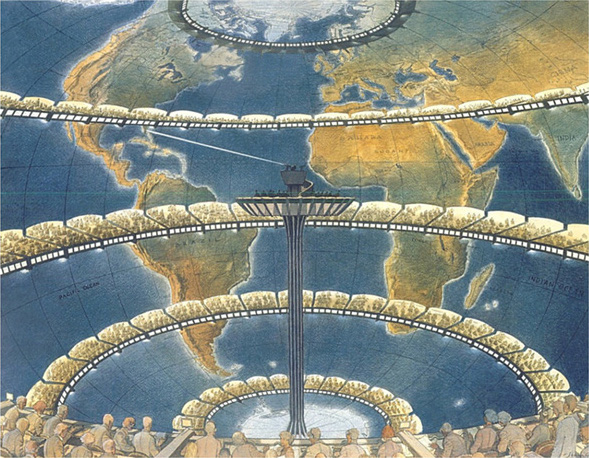
\includegraphics[width=\textwidth]{chapters/000-einleitung/images/forecast-factory-color.jpg}
\caption{Von Lewis Fry Richardson erdachte Vision einer Forecast-Factory
\label{buch:einleitung:fig:factory}}
\end{figure}
%
Er wendete die Methode der finiten Differenzen, die er 1911 in
\index{finite Differenzen}%
ganz anderem Zusammenhang entwickelt hatte, auf diese Grössen an.
Zur Durchführung der Berechnung entwickelte er eine Reihe von
Formularen, die die Daten und Zwischenresultate enthielten.
Für die praktische Realisierung hat er sich vorgestellt, dass 
eine grosse ``Berechnungsfabrik'' gebaut werden soll, in der 
``Computer'' mit seinen Formularen für jeden Punkt des Gitters 
Berechnungen anstellen und ihre Resultate den Nachbarn weitergeben
(Abbildung~\ref{buch:einleitung:fig:factory}).

Obwohl die Resultate, die Richardson erhalten hat, nicht korrekt waren,
hat sein Ansatz alle modernen Wettervorhersagemodelle beeinflusst%
\footnote{Eine umfassende Diskussion der Resultate von Richardson sowie
eine Einordnung in den Kontext seiner Zeit findet der Leser in der
hervorragenden Darstellung der historischen Darstellung \cite{buch:lynch}
von Peter Lynch.}.
Man kann ihn als den Vater der modernen numerischen Wetterprognose
bezeichnen.
Er basiert darauf, die Atmosphäre als sieben Felder zu betrachten,
sie auf Gitterpunkten zu diskretisieren und die sieben Feldgleichungen,
die die Variablen miteinander verbinden, numerisch zu lösen.
Die Wetterphänomene sind also ein Resultat des lokalen Atmosphärenzustands.
Änderungen dieses Zustands erfolgen durch den unmittelbaren Austausch
von Materie, Enerie und Impuls mit der unmittelbaren Umgebung.

Die Idee des Feldes gibt also das naheliegende physikalische Prinzip
wieder, dass physikalische Wirkung lokal stattfindet.
\index{Feld}%
Wärme wird durch Kontakt mit einem Körper anderer Temperatur übertragen,
Schallwellen transportieren Energie durch Stösse zwischen Luftmolekülen.
\index{Temperatur}%
Dies erfordert aber eine Revision der Newtonschen Ideen zur
Gravitation.
Es war schon Newton bewusst, dass sein Gravitationsgesetz eine 
Fernwirkung über riesige Distanzen beschreibt, ohne ein dazwischenliegendes
Medium, dass die Wirkung vermitteln könnte.
Eine ähnliche Schwierigkeit hat er auch bei Licht erkannt.
Trotz Hinweisen auf eine Wellennatur des Lichtes favorisierte Newton
eine Erklärung des Phänomens durch Partikel.
Erst im 19.~Jahrhundert wurde klar, dass das elektromagnetische Feld
die physikalische Entität ist, die Licht und alle anderen Arten von
elektromagnetischen Phänomenen transportieren kann.
Damit war der Begriff des Feldes nicht mehr nur eine mathematische
Spielerei sondern ein physikalisches Konzept, welches für alle Arten
von Wechselwirkungen anwendbar ist.

Die Physik des 20.~Jahrhunderts hat die Entwicklung der Feldtheorie als
zentrales physikalisches Paradigma mit zwei wesentlichen Entdeckungen
gekrönt.
Die erste war die Entdeckung Albert Einsteins, dass die Gravitationskraft
\index{Einstein, Albert}%
durch ein Feld vermittelt wird, welches in jedem Punkt die Längenmessung
beschreibt.
Er konnte für das metrische Feld Gleichungen aufstellen, welche die
Krümmung mit dem Energie- und Impulsgehalt des Raumes verknüpfen.
\index{Krümmung}%
Damit war Newtons Problem der Fernwirkung der Gravitation aus der Welt
geschafft.
Die zweite Entwicklung fand in der Mitte des Jahrhunderts statt.
Aus der Quantenmechanik entwickelte sich die Quantenfeldtheorie, die
alle Materieteilchen und Interaktionen durch Felder beschreibt.
Damit waren alle physikalischen Phänomene in letzter Konsequenz auf
Felder zurückgeführt.

